% This Labbook describes the development of mismatch models of CORN
% Zheng Hu and Sherry Dongqi Bao
% Created July 2018
% Last change July 2018


\documentclass[a4paper,10pt]{article}


\usepackage{lineno,hyperref}
\usepackage[utf8]{inputenc}
\usepackage{bm}
\usepackage{amsmath}
\usepackage{amssymb}
\usepackage{amssymb}
\usepackage[pdftex]{graphicx}
\usepackage{xcolor}
\definecolor{darkblue}{rgb}{0,0,0.5}
\usepackage{transparent}
\usepackage{algpseudocode}
\usepackage{algorithm}
\usepackage{hyperref}
\usepackage{graphicx}
\usepackage{subcaption}
\usepackage{pdfpages}
\usepackage{float} % added to avoid table movement
\usepackage{indentfirst} % added to indent first paragraph

\usepackage{cite}

\usepackage[backend=bibtex, style=numeric, sorting=none]{biblatex}
\usepackage{csquotes}
\addbibresource{reference.bib}

\usepackage{titlesec}
\setcounter{secnumdepth}{4}
\titleformat{\paragraph}
{\normalfont\normalsize\bfseries}{\theparagraph}{1em}{}
\titlespacing*{\paragraph}
{0pt}{3.25ex plus 1ex minus .2ex}{1.5ex plus .2ex}


\graphicspath{ {Figures/} }
\newcommand{\red}[1]{\textcolor{red}{#1}}
\newcommand{\green}[1]{\textcolor{green}{#1}}
\newcommand{\magenta}[1]{\textcolor{magenta}{#1}}
\renewcommand*\rmdefault{iwona}
%openings
\DeclareMathOperator*{\argmax}{arg\,max}

\title{Construction of Free Energy Model}
\author{Zheng Hu, Sherry Dongqi Bao \\ Tianjin University}

\begin{document}
	\maketitle

	\begin{abstract}
	Our model aims to find the intricate reason in gene cleaving behavior and find efficient method to enhance the genome-editing tools reliability, i.e. reducing the off-targeting possibility.
	The basic knowledges of this model are mostly simple probability and dynamic deduction, which make our model both convincing and pellucid.
	\end{abstract}
	
	%\input{miscorn_intro.tex}
	%\input{miscorn_methods.tex}
	
	%\section*{References}
	\addcontentsline{toc}{chapter}{Bibliography}
	\printbibliography
	%\chapter{existing model}
	\section{Introduction}
	In the appearing researching, people have construction similar model as illustrating in the following figure (Figure.1). There are four common rules when cas nuclease cleave the DNA \parencite{KLEIN20181413} 
	.
		\begin{figure}[tbph]
		\centering
		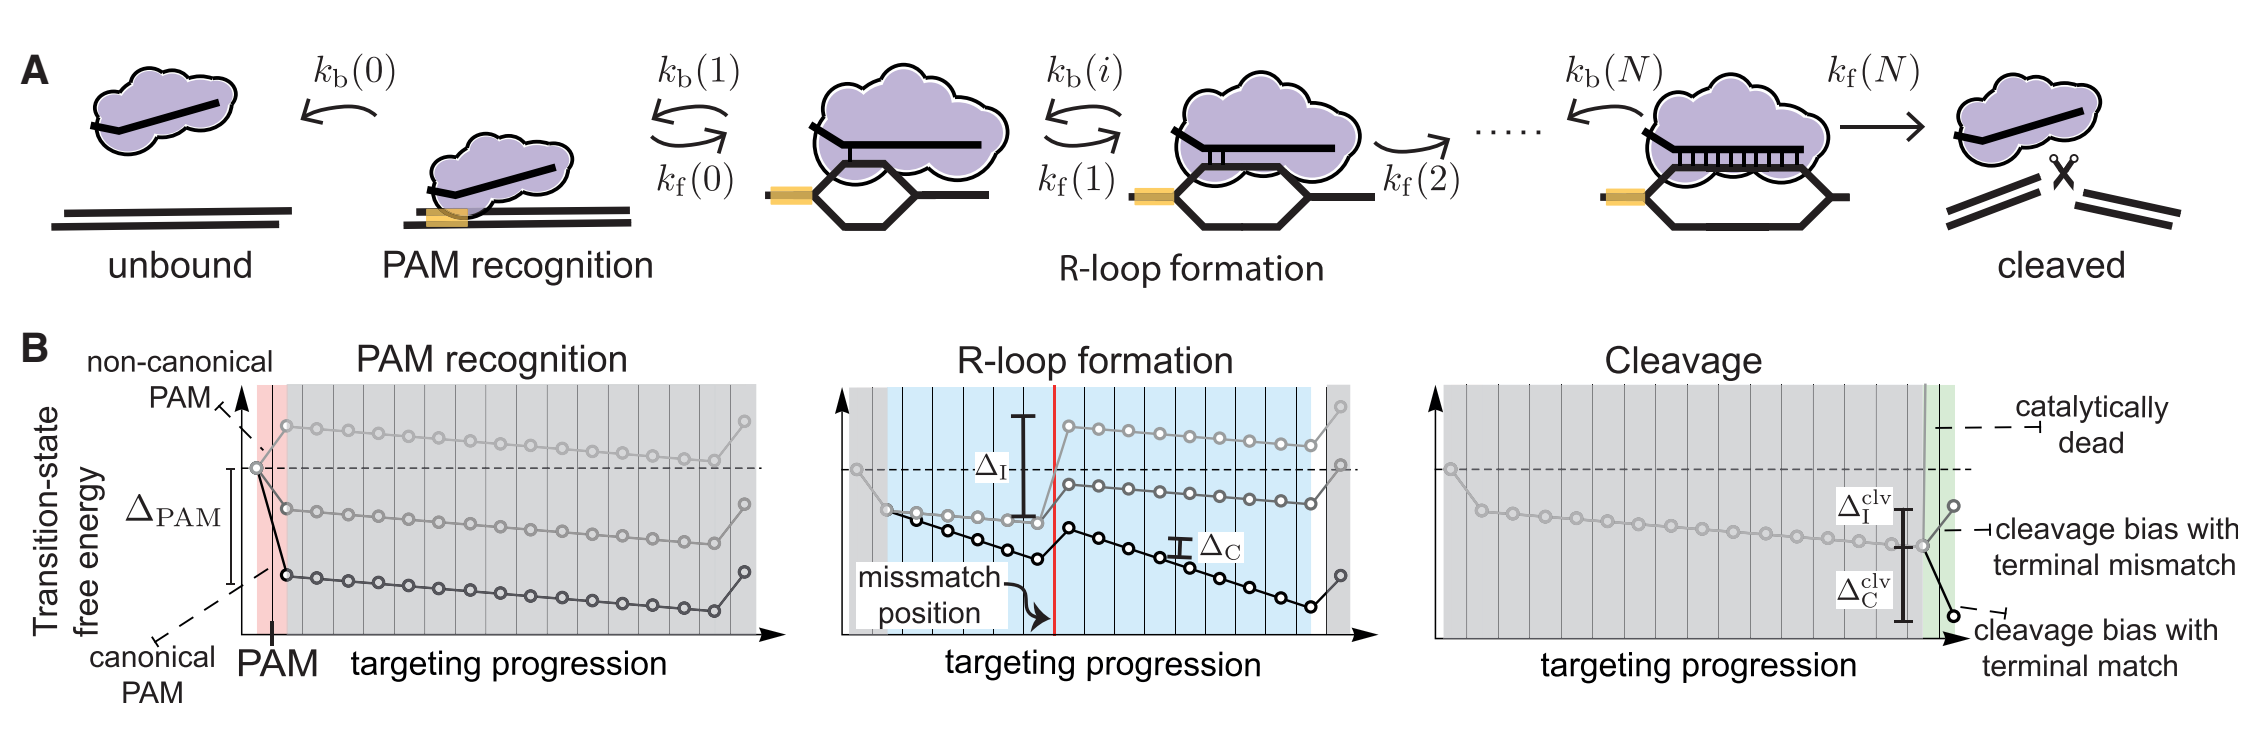
\includegraphics[width=3.5in]{1}
		\caption{schematic diagram}
		\label{fig:1}
		\end{figure}

	(1) seed region: single mismatches within a PAM proximal seed region can completely disrupt interference\par
	(2) mismatch spread: when mismatches are outside the seed region, off targets with spread out mismatches are targeted most strongly\par
	(3) differential binding versus differential cleavage: binding is more tolerant to mismatches than cleavage\par 
	(4) specificity-efficiency decoupling: weakened protein-DNA interactions can improve target selectivity while still maintaining efficiency\par
	Based on these four rules, possibility theory was applied in to explain it. As we know, there are always only two results in experiment, which are successful cleavage and unsuccessful cleavage. In math view, it can be on-hot encoded and they are corresponding to 1 and 0. To solve it, we may consider it as a cluster problem, however, it is easier to find a quantitative continuous function rather than try hard to find a suitable cluster distance function. Naturally, finding an approximate possibility distribution is a good choice. In many target design toolkits, they have a set of parameters to get a score to evaluate whether it’s good or bad. Here we think the score function has similar ability to possibility which is a description of better or worse and can’t affirm whether successful cleavage appear. Considering this problem, it roots in the question itself because future can’t be predicted. But possibility can. Hence, there we tend to find a function so that we can know what target is better.\par
	Considering difference between model predicting data and experimental data, our model consists of two aspects, which are kinetic inference and updating module.
	\section{Model}
	%	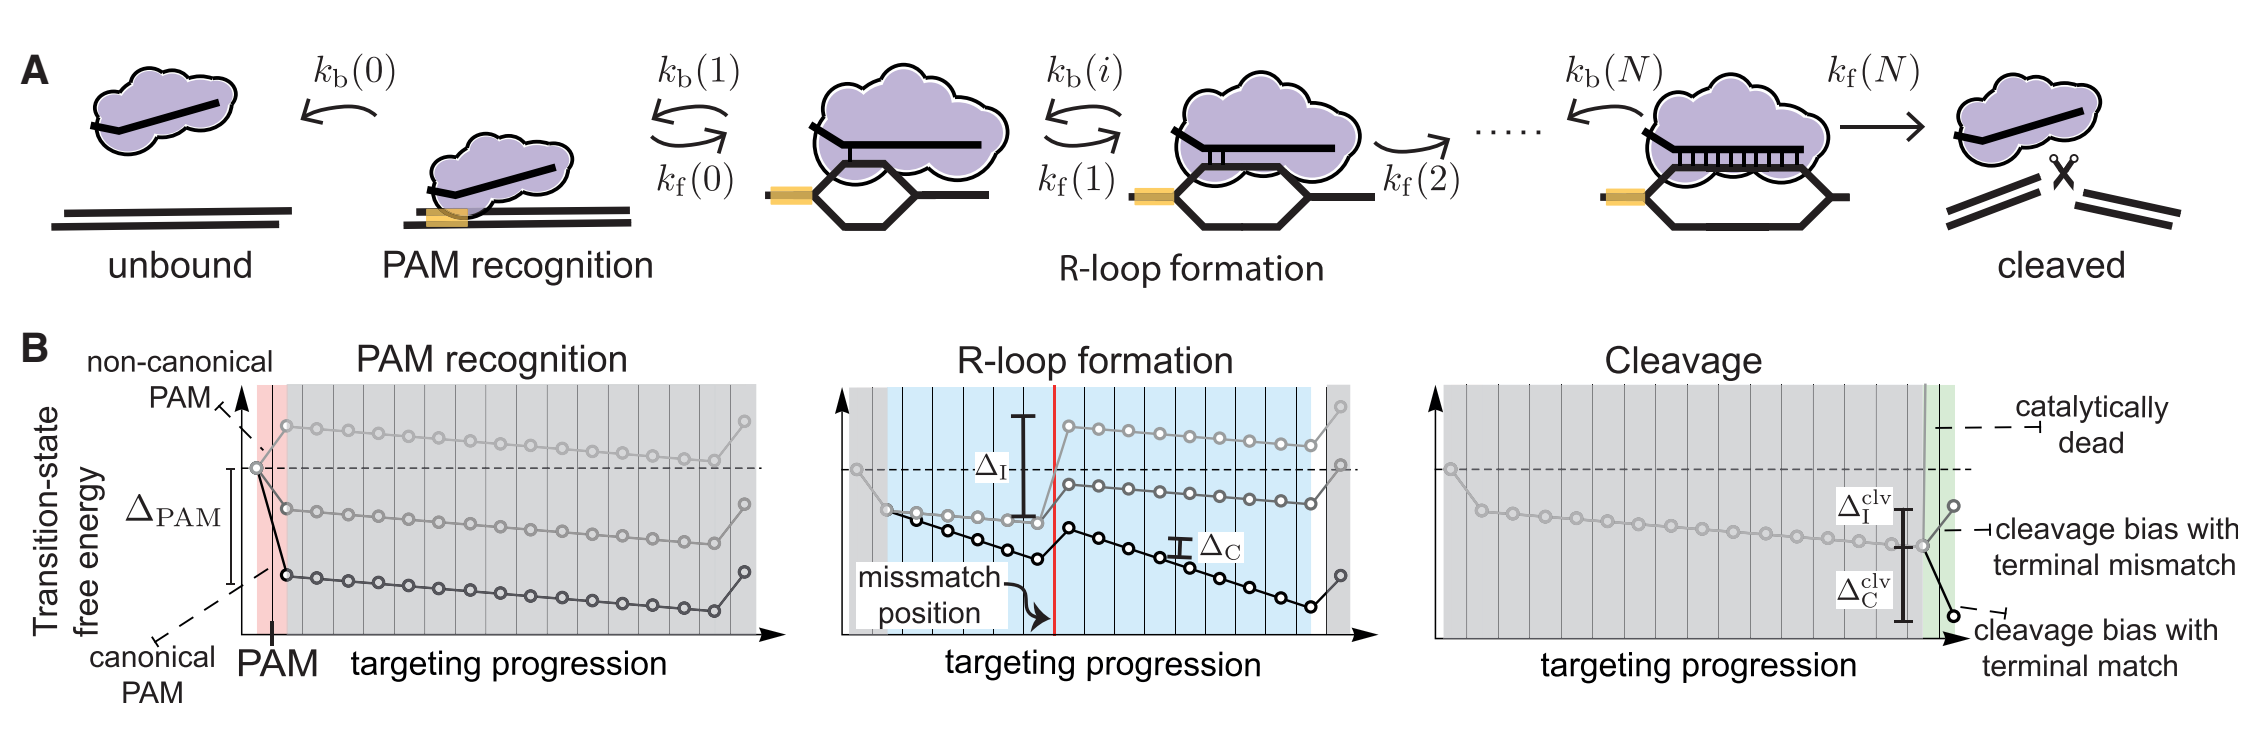
\includegraphics[width=5in]{1.png}
	\subsection{kinetic model}
	From the figure.2, this process is begun with binding between PAM and protein. Therefore, it corresponds to rule 1 mentioned before. And with the reaction proceeding, every steps in it are reversible and it’s irreversibility mainly depended on the banding energy of two DNA bases.
	\begin{figure}
		\centering
		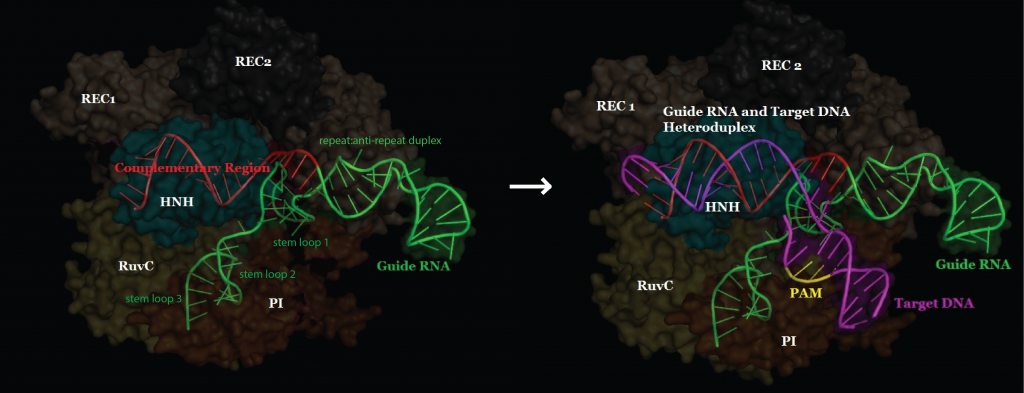
\includegraphics[width=0.7\linewidth]{2}
		\caption{}
		\label{fig:2}
	\end{figure}
	\begin{figure}
		\centering
		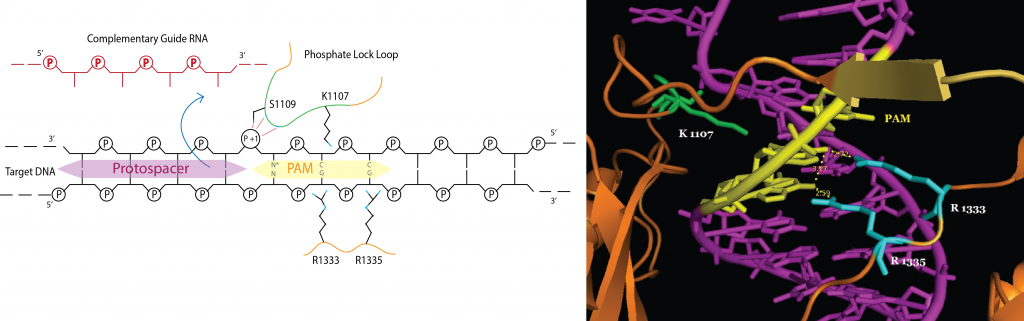
\includegraphics[width=0.7\linewidth]{3}
		\caption{}
		\label{fig:3}
	\end{figure}
	\begin{figure}
		\centering
		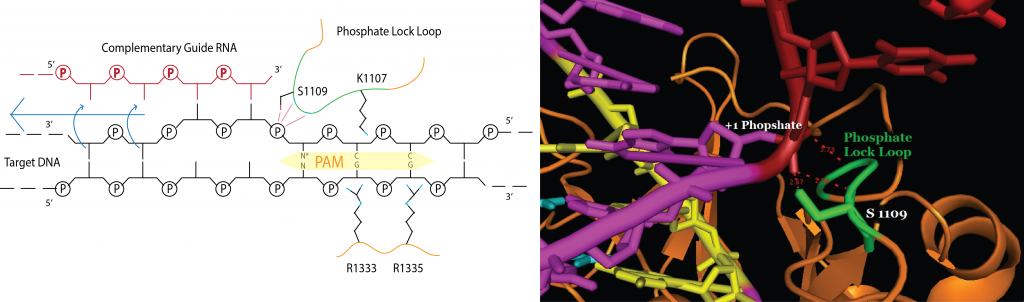
\includegraphics[width=0.7\linewidth]{4}
		\caption{}
		\label{fig:4}
	\end{figure}
	\begin{figure}
		\centering
		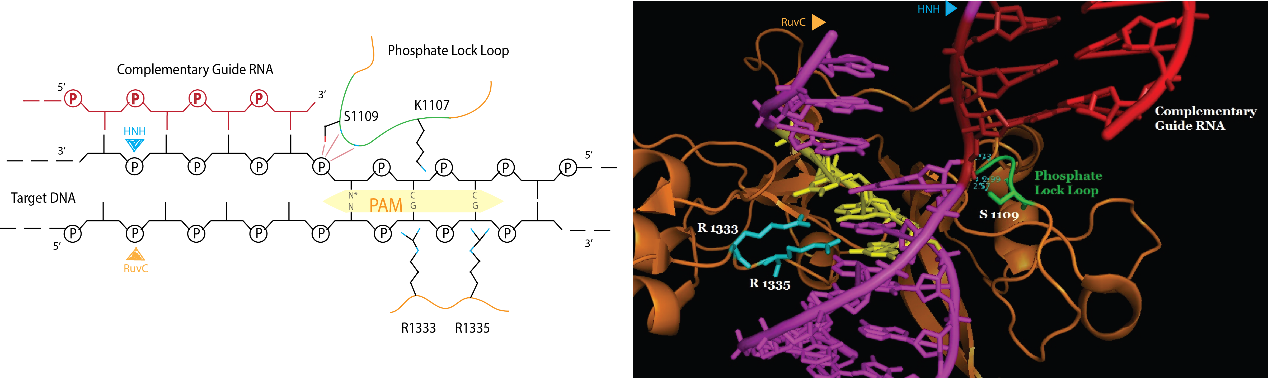
\includegraphics[width=0.7\linewidth]{5}
		\caption{}
		\label{fig:5}
	\end{figure}
	
	The boundary probability Pclv;N , representing the probability to cleave staring with a full R-loop and
	without reducing the R-loop’s length, is given by a simple splitting probability:
	$$P_{clv,N}=\frac{k_f(N)}{k_f(N)+k_b(N)}=\frac{1}{1+\gamma_N} \quad \gamma_N=\frac{k_b(N)}{k_f(N)}$$
	$$P_{clv} \equiv P_{clv,0} = \frac{1}{1+\sum_{k=1}^N\coprod_{i=1}^n \gamma_i} $$
	free-energy:$F_i$ ; the transition state energy:$T_i$, from $i$ to $i+1$, we can get the relationship between reaction constant and free energy:
	$$k_f(i)=k_0exp(-(T_i-F_i)),k_b(i)=k_0exp(-(-T_{i-1}-F_i))$$ $$\Rightarrow \gamma_i=exp(-\Delta_i),\Delta_i=T_i-T_{i-1}$$
	$$\Rightarrow P_{clv} = \frac{1}{1+\sum_{k=1}^N\coprod_{i=1}^n \gamma_i}=\frac{1}{1+\sum_{k=1}^N\coprod_{i=1}^n exp(-\Delta_i)}=\frac{1}{1+\sum_{k=1}^N exp(-\sum_{k=1}^n\Delta_i)} $$
	define: $$\Delta T_n=\sum_{k=1}^n\Delta_i$$
	$$ P_{clv} =\frac{1}{1+\sum_{k=1}^N exp(-\Delta T_n)}$$
	From the above it is clear that the cleavage probability depends only on the transition state energies,
	and not on the free energies of the metastable states. If we assume there to be one dominant minimal bias, say for $n = n^∗$, then this can be approximated as:
	$$ P_{clv} \approx \frac{1}{1+exp(-\Delta T_{n^∗})}$$
	As figure shows, we analyse each process energy change:\newline
	$\left\{
	\begin{tabular}{l}
	for the PAM state (i = 0) we have 
	$\Delta_0=∆PAM$\\
	for a partial R-loop we have $\Delta_i = \Delta_C$ and $\Delta_i = −\Delta_I$ if mismatched\\
	\end{tabular}
	\right.$
	$$\Delta T_n =\Delta_{PAM} + n_C(n)\Delta_C − (n − n_C(n))\Delta_I − \delta_{n,N}\Delta_{clv}; n = 0 \dots N$$
	where $\delta_{n,N}$ represents the $Kronecker$ delta:
	$\delta_{n,N}$=$\left\{\begin{array}{l}1, n=N;\\
	0, n\neq N.
	\end{array}
	\right.$\\
	For PAM independent systems (such as cas13), we instead use:
	$$\Delta T_n =n_C(n)\Delta_{C} − (n−n_C(n))\Delta_{I} − \delta_{n,N}\Delta_{clv}; n = 0 \dots N$$
	To sum up, the cleavage possibility mainly rely on the free energy change, and PAM appears as a large energy decline.\par
	So the kenetic module set up a form to regression the relationship between cleavage and the numbers of nucleotide matches and mismatches.
	Considering this problem more carefully, the cleavage possibility become equal to analysis energy change and simply we know the binding energy of A/T and C/G is different due to the different hydrogen bond between them. However, in appearing kinetic model, research tend to describe them in a rough definition as “matched base pairs” and the energy incline in C/G is approximately 1.5 folds as A/T. Similarly, the mismatch has more difference because the size of nucleotides is various. Hence, the combination of mismatched base pair was classified by group volume, i.e. two pyrimidine (such as C/T, “L”), pyrimidine  and purine (such as C/A, “M”), two purine (such as G/T, “S”). Hence, our possibility can be calculated using following formation.
	$$
	P_{clv}=\frac{1}{1+e^{-n_1\Delta_{A/T}-n_2\Delta_{C/G}+n_3\Delta_{L}+n_4\Delta_{M}+n_5\Delta_{S}}}
	$$
	\subsection{Optimization model}
	It is common sense that experiment result are facts but theorical results are only conjectures. In the model 1, we can get an output, which means the cleavage possibility. The parameter we chooce only aim to make results has discrimination, while it’s not quantitative. And in a cleavage experiment, we only have two results, successful and unsuccessful. To make our prediction possibility more approximate to experiment, we regard this as a regression problem.\par
	Here, the method we choose is stochastic gradient descent (SGD) and choose cross entropy. And their principle can be concluded as following.
	\[\theta  = \theta  - \eta {\nabla _\theta }J({x^{(i)}},{y^{(i)}},\theta )\]
	\[loss = \sum\limits_i {{y_i}\ln {y_i}}\]
	where $\theta$ means the parameters array and J means the loss function, \par
	Considering the difference in gradient calculation, we use difference to substitute differential aim to accelerate operating speed.\par
	\[\frac{{dy}}{{dx}} \approx \frac{{\Delta y}}{{\Delta x}}{\rm{ = }}\frac{{y(x + \delta x) - y(x)}}{{\delta x}}\]
	By using this simple method, our model can be more vibrant, updating using newest data and becoming more reliable.
	\subsection{Pre-selector}
	It’s obviously that the algorithm is too complex to applying in slide in a huge DNA array. To solve this problem, we use a pre-selector to get some candidates and use previous model to compare them so that we could get a greatest target.\par
	And here this pre-selector structure is very simple.
	Considering use this map to reflect the similarity between target and full DNA.
	\[f({a_{{\rm{target}}}} - {a_{{\rm{full}}}}) = {\bf{x}} = ({x_i})\]
	\[{x_i} = \left\{ {\begin{array}{*{20}{c}}
		{1,\quad \quad matched}  \\
		{0,\quad mismatched}  \\
		\end{array}} \right.\]
	Here, we use PAM as an input and collect the array which contain the same beginning code as PAM.
	\section{Result}
	Here, we set this parameters as default values and observe its performance. As the following figure shows, the energy is always declined or has some turning point and is alway negative. Such as the red line, it have a peak due to a mismatch here, and in our model we find that it doesn't make the energy positive. That means that in this reaction process there are some force somewhat like momentum pushing it proceed and cross the energy peak. Corresponing to the other figure's two special location(a ad b), only in these point their energy are all negative (because we want to see the idea target series, only the locaitons which corresponds to negative energy are collected).\par
\begin{figure}[h]
	\centering
	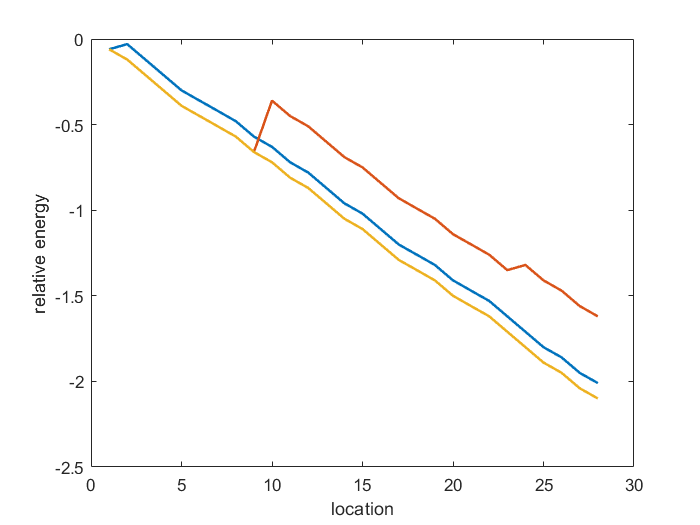
\includegraphics[width=0.7\linewidth]{energy_change}
	\caption{energy change}
	\label{fig:energychange}
\end{figure}
\begin{figure}[h]
	\centering
	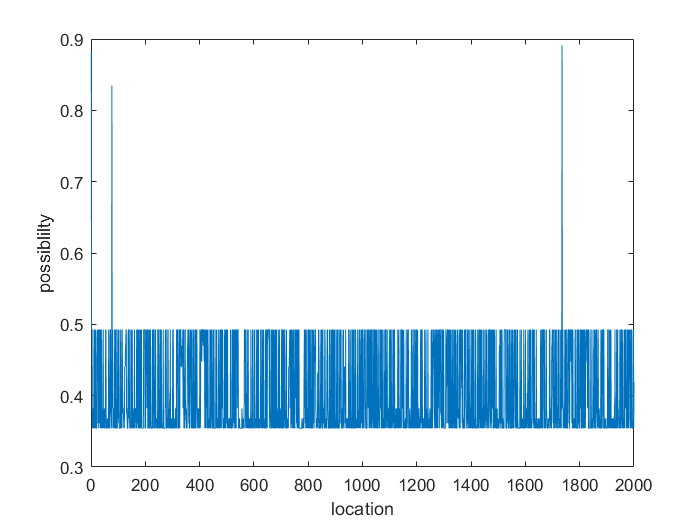
\includegraphics[width=0.7\linewidth]{fig1}
	\caption{the possibility of target binding to nucleotide array in different location}
	\label{fig:fig1}
\end{figure}
Besides the default parameters, we hope our model can hit more ture data. So if we get the experiment datas, we can use model 2.2 to get greater parameters.(@@no experiment data) 
\bibliographystyle{abbrv}	
\bibliography{cited}


\end{document}
